\chapter{METHODOLOGY}

\section{Preprocessing}

The preprocessing pipeline is the same as in the first phase (EE491). All recordings are sampled at $F_s = 4800$\,Hz. The following channel-specific filters are applied using 4th-order Butterworth filters with zero-phase (forward--backward) filtering:

\begin{table}[H]
\centering
\caption{Per-channel filter configuration.}
\label{tab:filters}
\begin{tabular}{@{}llll@{}}
\toprule
\textbf{Channel} & \textbf{Filter} & \textbf{Cutoff} & \textbf{Purpose} \\
\midrule
Pulmonary mic & Bandpass & 60--2200\,Hz & Retain cough band, remove drift and hum \\
Ambient mic   & Bandpass & 60--2200\,Hz & Same filter for fair channel comparison \\
Stretch sensor & Low-pass & 20\,Hz & Retain slow chest movement \\
Accelerometer  & Low-pass & 20\,Hz & Preserve DC (gravity) and gross motion \\
\bottomrule
\end{tabular}
\end{table}

Before filtering, the stretch sensor channel is decoded using bitwise operations (Equations~\ref{eq:label}--\ref{eq:stretch}). Audio signals are median-centered. Motion signals (stretch and accelerometer Z-axis) are resampled from 4800\,Hz to 100\,Hz after low-pass filtering.

\section{Windowing and Labeling}

Continuous signals are segmented into overlapping windows of 1.0\,s duration. The window size was chosen to be larger than in the previous phase (200\,ms) to give the CNN models more temporal context. Two labeling strategies were used across the three model versions:

\begin{itemize}[nosep]
    \item \textbf{V1 labeling:} A window is labeled as cough-positive if \emph{any} cough label exists within the full window. The hop size is 0.5\,s.
    \item \textbf{V2/V3 labeling:} A window is labeled as cough-positive only if a cough label exists in the \emph{center 20\%} of the window. The hop size is reduced to 0.25\,s.
\end{itemize}

Figure~\ref{fig:windowing} illustrates the difference between these two strategies.

\begin{figure}[H]
\centering
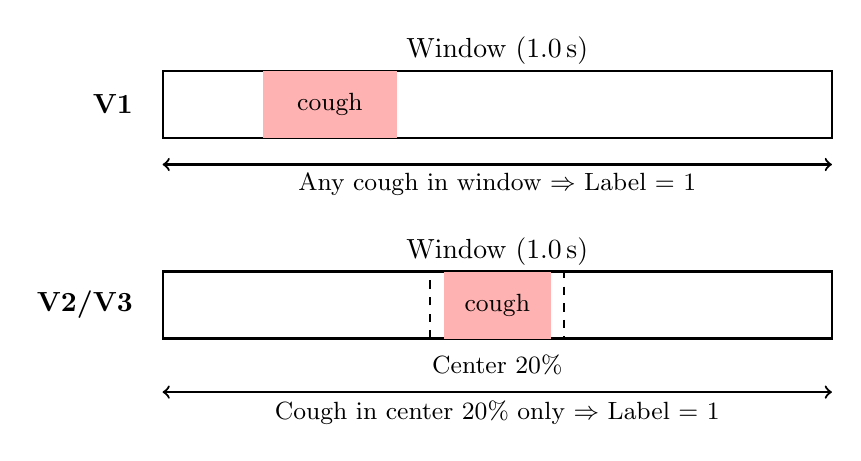
\begin{tikzpicture}[scale=0.85]
    % V1 labeling
    \node[anchor=east] at (-0.3, 1.5) {\textbf{V1}};
    \draw[thick] (0, 1) rectangle (10, 2);
    \node at (5, 2.3) {Window (1.0\,s)};
    \fill[red!30] (1.5, 1) rectangle (3.5, 2);
    \node[font=\small] at (2.5, 1.5) {cough};
    \draw[thick, <->] (0, 0.6) -- (10, 0.6);
    \node[font=\small] at (5, 0.3) {Any cough in window $\Rightarrow$ Label = 1};

    % V2/V3 labeling
    \node[anchor=east] at (-0.3, -1.5) {\textbf{V2/V3}};
    \draw[thick] (0, -2) rectangle (10, -1);
    \node at (5, -0.7) {Window (1.0\,s)};
    \draw[dashed, thick] (4, -2) rectangle (6, -1);
    \node[font=\small] at (5, -2.4) {Center 20\%};
    \fill[red!30] (4.2, -2) rectangle (5.8, -1);
    \node[font=\small] at (5, -1.5) {cough};
    \draw[thick, <->] (0, -2.8) -- (10, -2.8);
    \node[font=\small] at (5, -3.1) {Cough in center 20\% only $\Rightarrow$ Label = 1};
\end{tikzpicture}
\caption{Comparison of V1 and V2/V3 window labeling strategies.}
\label{fig:windowing}
\end{figure}

The center labeling strategy reduces the number of windows that are labeled as positive only because a cough event partially overlaps with the window boundary. This provides cleaner labels for training, at the cost of labeling fewer windows as positive.

Each window produces two input tensors: an audio tensor of shape $(2, 4800)$ containing the pulmonary and ambient microphone signals, and a motion tensor of shape $(2, 100)$ containing the stretch and accelerometer signals.

\section{Model Architecture}

All three model versions follow a dual-branch architecture with late fusion. Two separate CNN branches process the audio and motion inputs independently. Their output embeddings are concatenated and passed through fully connected layers for classification. Figure~\ref{fig:architecture} shows the general architecture.

\begin{figure}[H]
\centering
\begin{tikzpicture}[
    block/.style={rectangle, draw, fill=blue!8, text width=2.2cm, text centered, minimum height=0.7cm, rounded corners=2pt, font=\small},
    blockG/.style={rectangle, draw, fill=green!8, text width=1.8cm, text centered, minimum height=0.7cm, rounded corners=2pt, font=\small},
    blockO/.style={rectangle, draw, fill=orange!8, text width=1.8cm, text centered, minimum height=0.7cm, rounded corners=2pt, font=\small},
    arr/.style={-{Stealth[length=2mm]}, thick},
    scale=0.9
]

% Audio branch
\node[block] (ain) {Audio input};
\node[block, right=0.6cm of ain] (acnn) {CNN layers};
\node[block, right=0.6cm of acnn] (apool) {Global pool};
\node[font=\small, right=0.3cm of apool] (adim) {64-d};

% Motion branch
\node[block, below=1.5cm of ain] (min) {Motion input};
\node[block, right=0.6cm of min] (mcnn) {CNN layers};
\node[block, right=0.6cm of mcnn] (mpool) {Global pool};
\node[font=\small, right=0.3cm of mpool] (mdim) {32-d};

% Fusion
\node[blockG, right=1.8cm of apool, yshift=-0.75cm] (cat) {Concat};
\node[blockO, right=0.6cm of cat] (fc) {FC + Out};

% Labels
\node[font=\footnotesize\itshape, above=0.1cm of ain] {V1/V2: 1D (2, 4800)};
\node[font=\footnotesize\itshape, above=0.1cm of acnn] {V1/V2: Conv1D};
\node[font=\footnotesize\itshape, below=0.1cm of min] {(2, 100)};
\node[font=\footnotesize\itshape, below=0.1cm of mcnn] {Conv1D};

% Arrows
\draw[arr] (ain) -- (acnn);
\draw[arr] (acnn) -- (apool);
\draw[arr] (apool) -- (adim);
\draw[arr] (adim.east) -- ++(0.3,0) |- (cat.west);
\draw[arr] (min) -- (mcnn);
\draw[arr] (mcnn) -- (mpool);
\draw[arr] (mpool) -- (mdim);
\draw[arr] (mdim.east) -- ++(0.3,0) |- (cat.west);
\draw[arr] (cat) -- (fc);

\end{tikzpicture}
\caption{General dual-branch architecture with late fusion. V1/V2 use 1D CNNs on raw audio waveforms. V3 replaces the audio branch with a 2D CNN on log-Mel spectrograms.}
\label{fig:architecture}
\end{figure}

\subsection{V1: Dual-Branch 1D CNN}

The V1 model (\texttt{DualBranchCoughCNN}) takes raw waveform inputs. The audio branch processes the 2-channel audio signal through three Conv1D layers with increasing channel counts ($2 \to 16 \to 32 \to 64$), each followed by batch normalization, ReLU, and max pooling. A global adaptive average pooling layer reduces the output to a 64-dimensional embedding.

The motion branch has a similar but smaller structure: two Conv1D layers ($2 \to 16 \to 32$) followed by adaptive average pooling, producing a 32-dimensional embedding.

The two embeddings are concatenated (96 dimensions) and passed through a classifier: Linear($96 \to 64$) $\to$ ReLU $\to$ Dropout(0.3) $\to$ Linear($64 \to 1$). The output is a single logit for binary cough detection.

\subsection{V2: Enhanced Training Strategy}

The V2 model uses the same \texttt{DualBranchCoughCNN} architecture as V1. The improvements are in the training process:

\begin{itemize}[nosep]
    \item \textbf{Data augmentation:} Additive white Gaussian noise (AWGN) is applied to both audio and motion tensors during cough detection training. For activity classification (Phase~2), synchronized circular time shifts are additionally applied.
    \item \textbf{Learning rate scheduling:} \texttt{ReduceLROnPlateau} monitors the validation loss and reduces the learning rate by half after 3 epochs without improvement.
    \item \textbf{Center labeling:} As described in Section~4.2, only cough labels in the center 20\% of the window count as positive.
    \item \textbf{Longer training:} The number of epochs is increased from 15 to 25.
\end{itemize}

\subsection{V3: Spectrogram-Based Model}

The V3 model (\texttt{Spec2DCoughCNN}) changes the audio input from raw waveforms to log-Mel spectrograms. The spectrogram is computed using the following parameters:

\begin{itemize}[nosep]
    \item FFT size: $N_{\text{FFT}} = 512$
    \item Hop length: 128 samples
    \item Mel bands: $N_{\text{MELS}} = 64$
    \item Frequency range: 60--2200\,Hz (matching the audio bandpass filter)
\end{itemize}

The resulting spectrogram has shape $(2, 64, 38)$ for 2 channels, 64 Mel bands, and 38 time frames per 1-second window. A logarithmic transformation is applied: $\log(\text{mel} + 10^{-9})$.

The audio branch uses three Conv2D layers ($2 \to 16 \to 32 \to 64$ channels) with $3 \times 3$ kernels, batch normalization, ReLU, and max pooling. Adaptive average pooling produces a 64-dimensional embedding. The motion branch remains unchanged from V1/V2.

An example log-Mel spectrogram is shown in Figure~\ref{fig:melspec}.

\begin{figure}[H]
\centering

\includegraphics[width=0.8\textwidth]{mel_spectrogram_example.png}
\caption{Example log-Mel spectrogram of the pulmonary microphone channel (top) and the corresponding time-domain signal with ground truth cough labels (bottom). Cough events appear as broadband vertical patterns in the spectrogram.}
\label{fig:melspec}
\end{figure}

\section{Training Configuration}

Table~\ref{tab:training_config} summarizes the training configuration for Phase~1 (cough detection) across all three versions.

\begin{table}[H]
\centering
\caption{Phase~1 (cough detection) training configuration comparison.}
\label{tab:training_config}
\small
\begin{tabular}{@{}lccc@{}}
\toprule
\textbf{Parameter} & \textbf{V1} & \textbf{V2} & \textbf{V3} \\
\midrule
Audio input & Raw waveform & Raw waveform & Log-Mel spectrogram \\
Audio CNN & 1D & 1D & 2D \\
Window / hop (s) & 1.0\,/\,0.5 & 1.0\,/\,0.25 & 1.0\,/\,0.25 \\
Label rule & Full window & Center 20\% & Center 20\% \\
Optimizer & Adam & Adam & Adam \\
Learning rate & $10^{-3}$ & $10^{-3}$ & $10^{-3}$ \\
Weight decay & $10^{-4}$ & $10^{-4}$ & $10^{-4}$ \\
Epochs & 15 & 25 & 25 \\
Batch size & 64 & 64 & 64 \\
Loss & \multicolumn{3}{c}{BCEWithLogitsLoss} \\
\texttt{pos\_weight} & $\sim$3.1 & $\sim$4.8 & $\sim$4.8 \\
Augmentation & None & AWGN & None \\
LR scheduler & None & \multicolumn{2}{c}{ReduceLROnPlateau} \\
\bottomrule
\end{tabular}
\end{table}

All three versions use the Adam optimizer~\cite{kingma2015adam} with binary cross-entropy loss (BCEWithLogitsLoss)~\cite{goodfellow2016deep} for cough detection. The \texttt{pos\_weight} parameter compensates for class imbalance by weighting positive (cough) samples more in the loss function. It is computed as the ratio of negative to positive training windows. The higher value in V2/V3 reflects the stricter center labeling, which produces fewer positive windows.

\section{Activity Classification (Phase 2)}

After cough detection, a second model is trained for activity classification using the same dual-branch architecture but with a multi-class output head.

\begin{itemize}[nosep]
    \item \textbf{V1:} Only 2 classes (sitting and walking) are used. Only windows from cough-positive segments are included. The loss is cross-entropy~\cite{goodfellow2016deep}.
    \item \textbf{V2:} All 4 activity classes (sitting, walking, standing, running) are used. All windows are included regardless of cough presence. The loss is weighted cross-entropy with class weights, using AdamW optimizer~\cite{loshchilov2019adamw}.
    \item \textbf{V3:} Three activity classes (sitting, standing, walking) are used. Running is excluded because having only 5 running records makes reliable stratified splitting across train, validation, and test sets impractical. Stratified record-level splitting is applied to ensure balanced activity representation. Multiple runs (A--D) are conducted with different combinations of class weighting and weighted sampling to find the best configuration.
\end{itemize}

\section{Validation Strategy}

For Phase~1 (cough detection), data is split at the record level into training (70\%), validation (15\%), and test (15\%) sets using random splitting. This ensures that windows from the same recording do not appear in different splits. V1 used 71 records (train~49 / val~11 / test~11), while V2 and V3 used 85 records (train~59 / val~13 / test~13).

Unlike the GroupKFold cross-validation used in EE491, a single train/val/test split is used here. This choice is motivated by the higher computational cost of deep learning training, which makes repeated cross-validation impractical.

For Phase~2 (activity classification) in V3, a stratified split is applied based on record-level activity labels to ensure that each split contains a representative distribution of activities.
